 \chapter{Introduction}

 \section{Background and Motivation}
 
In the last decades, mortalities caused by heart diseases has been increasing sharply as a result of aging of population, chronic cardiovascular diseases, increasing life stress and continuously accelerating pace of life\cite{mortality}. According to heart disease and stroke statistics, cardiac diseases are the most common cause of sudden cardiac death (SCD) which leads to 250 000 to 300 000 mortalities in U.S. every year which accounts for 14.7\% of total deaths\cite{SCDnumber}. As World Health Organization reported, 31\% of global deaths are related to cardiovascular diseases (CVDs)\cite{who}. % Therefore, heart disease is called as “Plague of The Times”. In China, there are about 540,000 sudden cardiac deaths every year.In addition, heart diseases tend to attack younger generations, manifested by the increasing proportion of young patients.
These facts fully reflect that heart diseases are threatening the general health of human beings. Meanwhile since SCD can occur, most likely, without warning and apparent symptoms in advance, the prediction and early recognition of cardiac disease are considered challenging\cite{circulation2010}. Therefore it is of important significance to treat heart diseases timely by early detection and prediction of CVDs. 
While most CVDs are accompanied with arrhythmia, accurate and timely recolonization of arrhythmia is a key factor for preventing the incidence of heart diseases effectively and determine definitive therapies for CVDs.

Electrocardiogram (ECG),recorded for the first time by Waller in 1887, contains abundant physiological and pathological information that reflects the heart rhythm and status of various parts of the heart\cite{besterman1979waller}. %a professor of physiology at Queen Mary Hospital of Royal Society, by using the capillary electro-meter on hearts of dogs and human in 1887.
 ECG records signals generated by electrical activities of heart as a time series. As a noninvasive examination method, it is known to be highly reliable in reflecting functionality of heart. For this reason, ECG has become one of the most conventional technologies (ECG, clinical examination, radiation and ultrasonic inspection) in modernized hospitals and clinics, serving as an important reference for doctors’ diagnosis of heart diseases.


The traditional diagnosis based on ECG analysis are mainly accomplished manually by physicians. %According to working experiences and rich knowledge in heart diseases, experts observe and analyze ECG waveforms visually and make accurate diagnosis. 
However, this becomes costly and impractical when continuous monitoring for CVDs is required. There are tremendous ECG records generated everyday, all demand for timely diagnosis and analysis. Facing with the severe shortage of physicians, automatic ECG classification system is introduced to generate real-time analysis result and provide additional information to physicians. 

Automatic classification algorithms has been frequently investigated by researchers in the last decades. Whereas applying conventional classification algorithms on biomedical signals remains challenging, especially for applications of spontaneous disease detection. 

%0959-4965%
A typical feature of cardiovascular disease is its spontaneous occurrence. This unpredictability is the principal cause of high mortality for patients with heart disease. An informative anticipation of abnormality would enable a therapeutic intervention ahead of mortal occurrence and thus minimize risk of mortality. Nevertheless, the majority of developed conventional ECG classification systems haven't focused on real-time or predicting performance. %To address these problems, we propose in this thesis novel non-linear transformation based classification systems with the capacity to predict abnormality.

Another important character of ECG waveform is its variability caused by distinct physical conditions of different individuals (i.e. gender, age, body-mass index etc.)\cite{agesex}\cite{intervaria}. Conventional classification algorithms fall short of generalization when applying on different patients' records\cite{llamedo2012automatic}. Due to the inter-patient variation in ECG signals and the complexity of cardiac pathological information analysis, most of the existing ECG analysis software only serve as auxiliary devices for physicians. The final results of diagnosis still depend on manual labeling by cardiologists. %More importantly, the diagnostic accuracy of the automatic analysis system of the ECG signal still cannot reach the highest diagnostic accuracy of the clinician.

The automatic analysis of ECG signals incorporates a wide range of techniques. In this work, we focus on overcoming the two drawbacks of existing automatic ECG classification systems, which is patient-specificity and predicting capacity. This research aims at improving the inter-patient classification performance and predicting capacity of automatic analysis and recognition of arrhythmia with ECG signals, which has significance in efficient early detection of CVDs and reduce mortality rate of SCD. 

\section{ECG and Arrhythmia}

Electrocardiogram is widely used to monitor the electrical activities of heart and assist diagnosing fatal cardiac disease. In order to design algorithms specifically for ECG analysis, it's important to develop a insightful perception of the functionality of heart and ECG waveform.  

\subsection{Characteristics of ECG signal}

ECG signal reflects the periodical electric signals generated by heart. Fig.\ref{fig:cardiac_cycle} demonstrated the typical signal waveform for a cardiac cycle (i.e. a heartbeat), which is usually composed of three main waves: P wave, QRS complexes and T wave. These waves corresponds to different physiological activities of heart. P waves are generated by atrial depolarization which standards for the process of pumping blood to ventricles. QRS complexes as the most significant electric activities is caused by ventricular contraction meaning the process of pumping blood to lungs and the rest of the human body. Finally, T waves is the result of ventricular repolarization recovering this process at the end of a cardiac cycle. Accurate detection and segmentation of each waves are necessary for ECG analysis. The waves are usually localized at the peak of waves, these peaks are also called fiducial peaks. By detecting the most significant peak within QRS complexes: R peak, automatic algorithms are able to discriminate between two adjacent cardiac cycles. The interval between two R peaks is called RR interval, which is also the inverse of heart rate.

 \begin{figure}[t]
 	\centering
 	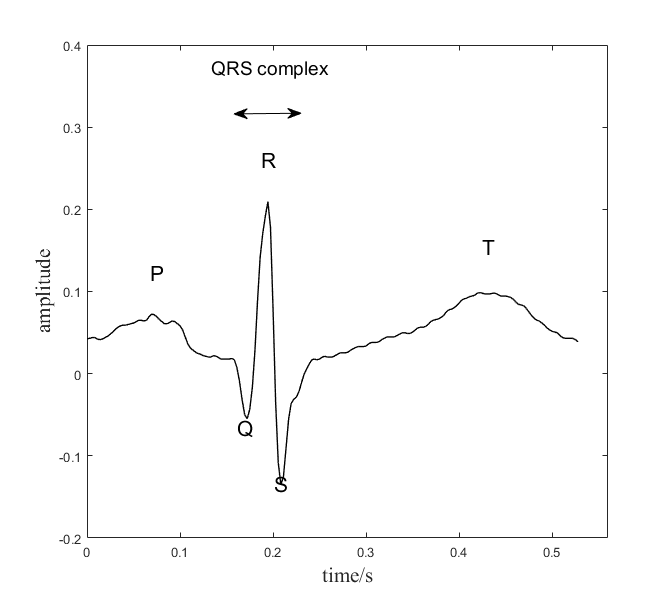
\includegraphics[scale=0.75]{Fig/cardiac_cycle.png}
 	\caption{A typical cardiac cycle in ECG signal with five characteristic waves}
 	\label{fig:cardiac_cycle}
 \end{figure}

\subsection{MIT-BIH Arrhythmia Database}

Arrhythmia is related to various of morbid behavior of heart. Generally speaking, arrhythmias consist of two main categories: supraventricular and ventricular. Ventricular ectopic beats imply abnormal activities in the ventricles while Supraventricular ectopic beats are related to the atria. Both categories contains fatal abnormal beats which may lead to death. Therefore, in order to help researchers standardize the evaluation of works on ECG classifiers, Association for the Advancement of Medical Instrumentation (AAMI) \cite{aami} has proposed recommendations for reporting ECG classifier performance. 
According to these recommendations, MIT-BIH Arrhythmia Database (MITDB) is regarded as the standard database to train and test ECG classifiers in the last decades. MITDB is a public database which is available on Physionet.com \cite{physionet} since 1997\cite{mitdb}. There are 48 records collected from 47 individuals in the database. Each record contains two channel of ECG raw signals together with annotations composed of 16 types and R peak locations provided by cardiologists. The sample frequency of MITDB is 360Hz and signal frequency spans from 0.1 to 100 Hz. 

Following the recommendation by AAMI, the original annotations of MITDB are further grouped into 4 major classes: class N(normal and bundle branch block beat types) class V(ventricular type), class S(supraventricular type) and class F(fusion of normal and ventricular types). The class Q which includes unclassified and paced beats are discarded due to the limit number of samples. Table.\ref{table:grouping_types} summarize the mapping from 16 original types in annotation to the standard 5 types recommended by AAMI:

\begin{table}[h]
\centering
\caption{Mapping from 16 original types in annotation to the standard 5 types recommended by AAMI}
\label{table:grouping_types}
\begin{tabular}{|c|c|}
\hline
Standard Types by AAMI & Original Types in MITDB Annotation \\ \hline
N                      & NOR, LBBB, RBBB, AE, NE            \\ \hline
V                      & PVC, VE, VF                        \\ \hline
S                      & APC, AP, BAP, NP                   \\ \hline
F                      & VFN                                \\ \hline
Q                      & PACE, FPN, UN                      \\ \hline
\end{tabular}
\end{table}



%For the purpose of training and evaluating classifier, MITDB is split into test (DS2) and training (DS1) set by balancing the four classes according to \cite{autofs}. 

\section{Problem Statement}

ECG signals, as a noninvasive method, are investigated broadly by researchers to design automated analysis and real-time monitoring systems. In the past decades, various ECG automatic analysis systems are proposed. As described in the last sections, there exists two main challenges: inter-patient variability and requirements for early detection and prediction. %To address these problems, we propose in this thesis two novel nonlinear transformation based patient-specific classification systems with the capacity to predict abnormality.

For conventional classification system, the training data is composed of records collected from different patients with annotations per heartbeat. In order to unify the records from different patients, most of the algorithms using conventional classification algorithm concatenate heartbeats from different records and thus result in a pooled ECG dataset. Since the classification performance is measured based on generated labels for each sample, the classifiers are trained to improve the performance on pooled ECG data. While ECG signals shares similar morphologies, the signals from different patients demonstrate considerable variance as shown in Fig.\ref{fig:interpatient_variability}. Ignoring this difference will lead to inconsistent classification performance between patients. Therefore it's of significant importance to adjust classifier configuration according to patient-specific characteristics.  %A patient-specific classification system refers to systems with cert

 \begin{figure}[thpb]
 	\centering
 	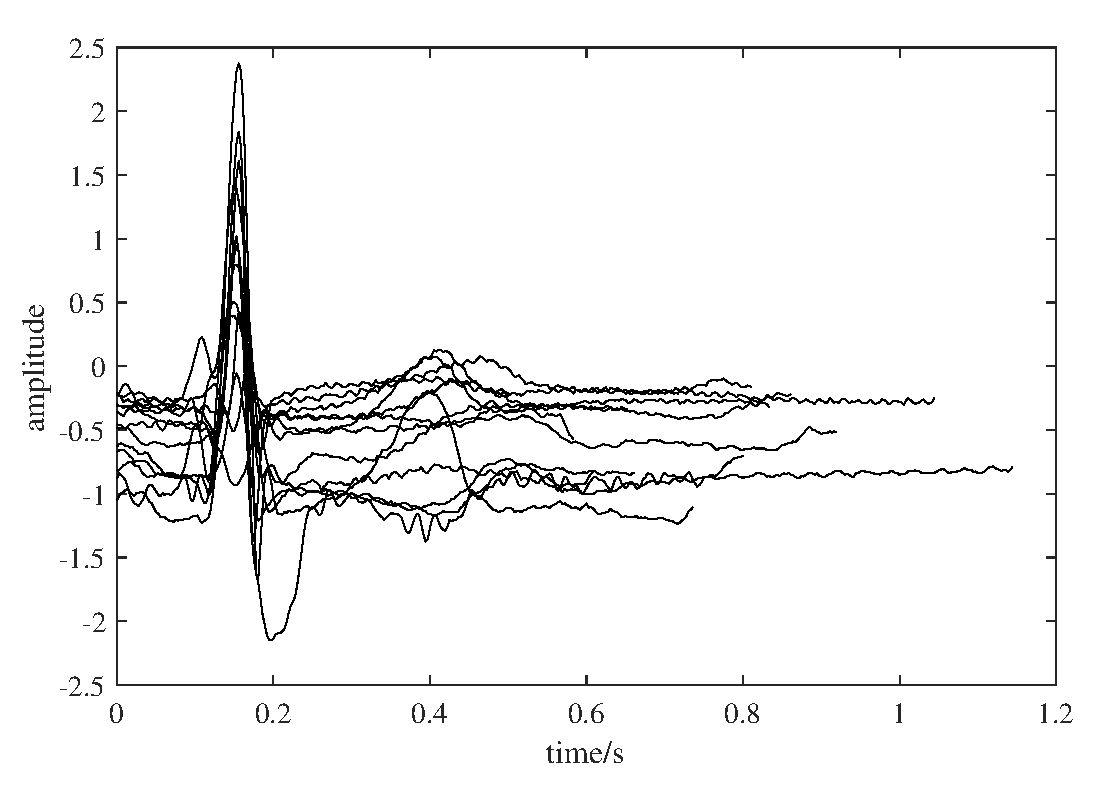
\includegraphics[scale=0.7]{Fig/interpatient_variability.pdf}
 	\caption{ECG signals of normal heartbeat from 15 different records reflect the inter-patient variability of ECG signal}
 	\label{fig:interpatient_variability}
 \end{figure}

In addition to the inter-patient variability, majority of ECG classification algorithms fail to consider the predicting capacity, which refers to the capacity of triggering corresponding alarms before the occurrence of abnormalities. By comparing the morphology of signals which shows salient similarities to abnormal signals precedent to morbid heartbeats with annotated abnormal signal, the potential latent status between abnormal and normal signals is partially demonstrated. If abnormalities in cardiologist annotation are represented by red alarms, thus a system which is able to trigger a corresponding yellow alarm precedent to the abnormality can be considered as capable of predicting abnormalities as shown in Fig.\ref{fig:pred_signals}. Therefore, a method to quantify the level of signal similarity to abnormalities should be incorporated in ECG classification system.

 \begin{figure}[t]
 	\centering
 	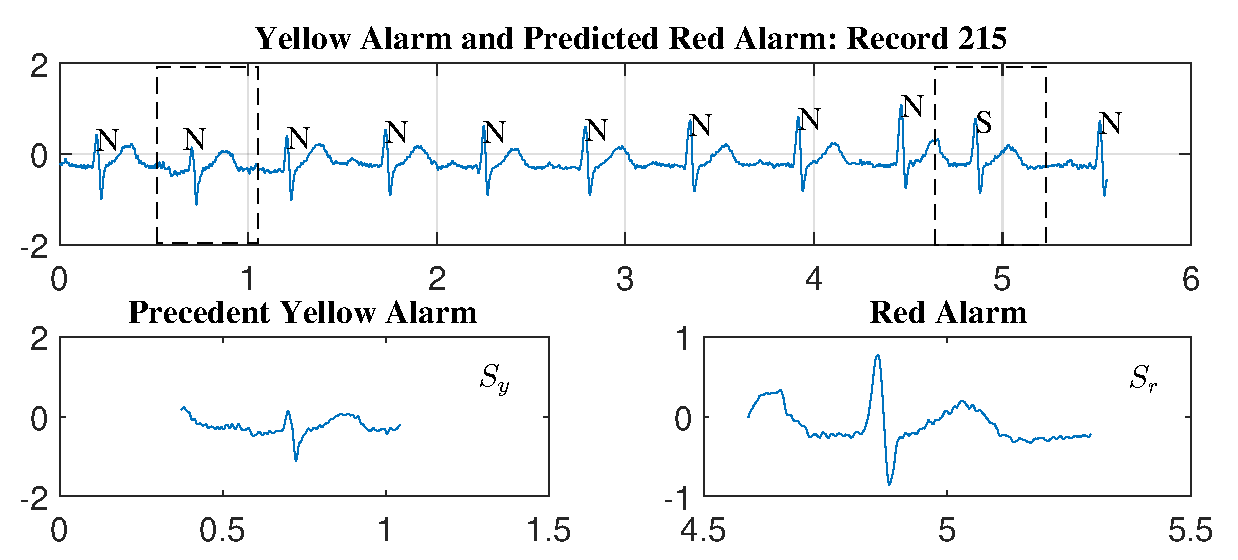
\includegraphics[scale=0.6]{Fig/predicting_record215S_croped.pdf}
 	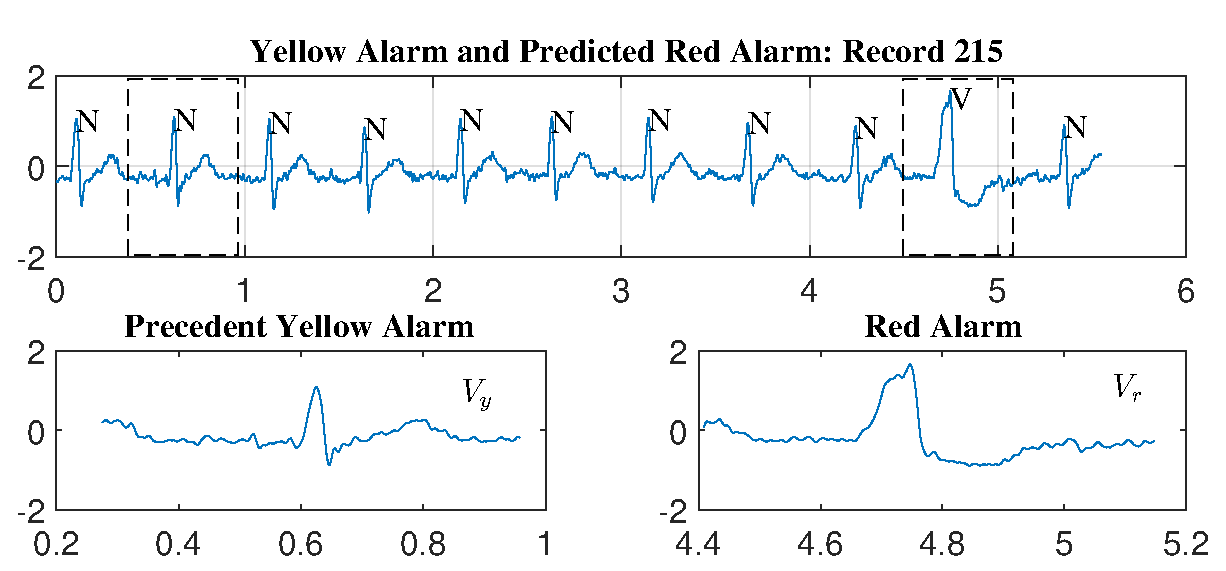
\includegraphics[scale=0.6]{Fig/predicting_record215_croped.pdf} 
 	\caption{Potential latent abnormal status(yellow alarm) predict upcoming abnormality of same type.}
 	\label{fig:pred_signals}
 \end{figure}




\section{Literature Review}
Automatic analysis of ECG signals refers to the entire process from acquisition of signals to classification of samples. This process can be divided into five stages: ECG signal acquisition, preprocessing, fiducial peak detection and segmentation, feature extraction, predictive modeling (Fig. \ref{fig:1-1}). There are researches focus on each single stage in the automatic analysis system. Since the main objectives of this work are addressing problems in classification algorithms, the literature reviews in this section focus on studying existing methods proposed for stages before classification, conventional classification algorithms along with patient-specific classification systems. 

 \begin{figure}[thpb]
 	\centering
 	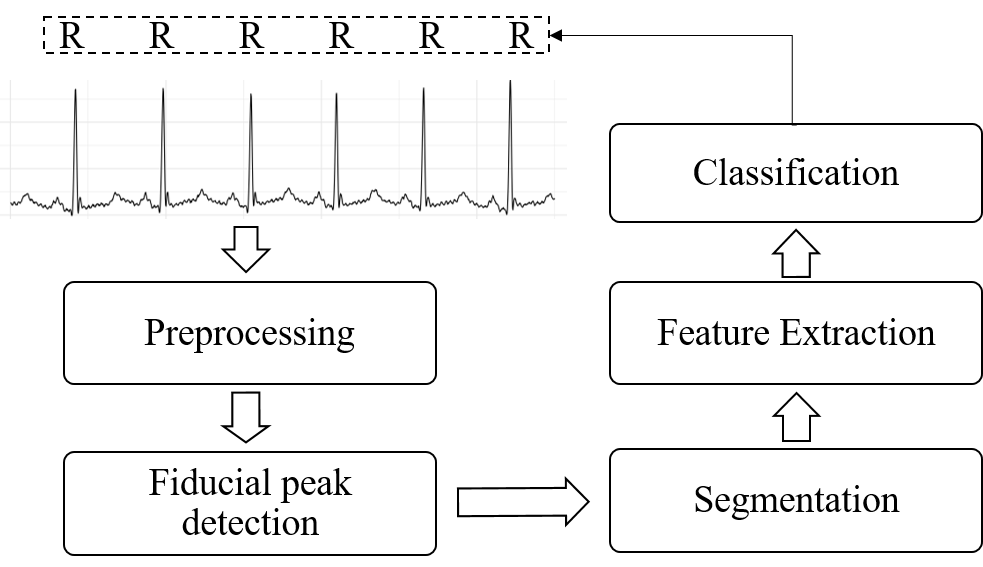
\includegraphics[scale=0.7]{Fig/general_flow.png}  
 	\caption{General structure of ECG classification system}
 	\label{fig:1-1}
 \end{figure}


\subsection{ECG Signal Preprocessing}

During data acquisition, ECG devices often introduce various noises including physiological noises (e.g. myoelectricity noise, breathe interference etc.) and non-physiological noises (e.g. power-frequency interference and electrode impedance interference) \cite{denoise}.These noises often interfere with informative signals and thus influence ECG classification results. Therefore ECG signal preprocessing mainly focus on the suppression of noise interference in ECG signals.

The ECG signal is in millivolt (mV) level with a frequency centered from 0 to 40 Hz\cite{thakor1984estimation}. Since ECG signal is comparatively weak with superposition of various noise, signal preprocessing is necessary step before classification. For this purpose, many researches have been conducted targeting different noise component in ECG signal.

Generally speaking, ECG signal preprocessing methods includes finite impulse response (FIR) filtering,   adaptive filtering, and modern signal processing filter methods such as wavelet transforms and neural networks. Ying -Wen Bai \textit{et al.} compared different notch filters and concluded that equiripple notch filter performs the best on ECG signal. Lian \textit{et al.} \cite{lian2004ecg} designed a multiplier-free finite impulse response (FIR) filters to surpress biological and environmential noises with a low cost of power consumption. Sayadi \textit{et al.} \cite{Sayadi} proposed a modified extended Kalman filter with estimated hidden state variables to perform denoising and compression at the same time. Park \textit{et al.}\cite{park1998application} designed a wavelet adaptive filter to reduce S-T segment distortion due to baseline drift and compared its performance with general adaptive filters. It is found that the wavelet adaptive filtering performance surpasses the general adaptive filters. In \cite{nikolaev2000wavelet}, the authors combined wavelet decomposition with Wiener filtering to filter noise by thresholding which is proved to outperform other thresholding denoising methods. Regarding various wavelet basis function, Singh \textit{et al.} studied the optimal selection of basis function for ECG signal denoising\cite{denoise}. By comparing the classification root mean square error using same classifier and different denoising methods, they concluded that Daubechies filter of order 8 performs the best for ECG classification system.


\subsection{Fiducial Peak Detection and Segmentation}\label{sec:fiducial_peaks}

Fiducial Peak Detection and cardiac cycle segmentation are the basis for extracting important information from ECG signals since a ECG record is usually a continuous time series so the information about single cardiac cycle can only be obtained after segmenting the records. The accuracy and reliability of this stage directly determine the final performance of diagnosis and analysis. 

Fiducial peak detection is also called ECG signal delineation, which aims at localize five characteristic peaks within one cardiac cycle. The most significant peaks are QRS complex consisting of Q, R and S peaks. The other two fiducial peaks are P wave before QRS complex and T wave after QRS complex. As shown in Fig.\ref{fig:fiducial_peaks}, these five characteristic waves along with the onset and offset of QRS complex are often used the depict a cardiac cycle.

 \begin{figure}[thpb]
 	\centering
 	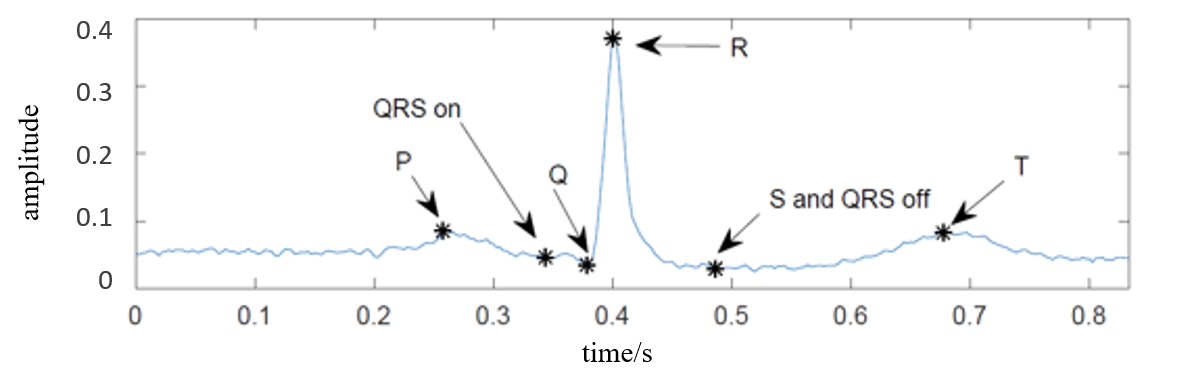
\includegraphics[scale=0.7]{Fig/fiducial_peaks.png}  
 	\caption{Fiducial peaks within one cardiac cycle}
 	\label{fig:fiducial_peaks}
 \end{figure}
 
As QRS complex is the most prominent waves and it contains most of the information of ECG signal, most of the methods for ECG delineation detect QRS complex prior to the detection of other peaks. Afonso \textit{et al.} \cite{afonso1999ecg} proposed a method using filter banks to detect QRS complex. In this method, signal is decomposed to several frequency band. Fiducial peaks are thus detected using its morphological features in the decomposed signals. Sadhukhan \textit{et al.} \cite{sadhukhan2012r} proposed a method of detecting R peak by comparing relative amplitude and double difference. The performance is validated on clinical ECG signal and proved to be promising. Some advanced machine learning techniques are also deployed to detect QRS complex. In \cite{mehta2008svm}, Support Vector Machine is used to train a predictive model for QRS complex detection and achived 99.93\% accuracy. Other pattern recognition models such as Hidden Markov Models are investigated and proved to be effecient in modeling and detecting characteritic peaks in ECG signals\cite{andreao2006ecg}. Wavelet decomposition is also frequently adopted for signal delineation for the morphological similarity between wavelet basis function and QRS complex. As the QRS complex power spectrum is centered at the range of 5 to 30 Hz, wavelet coefficients of corresponding scale levels are frequently used for delineation. In \cite{martinez2004wavelet}, QRS complexes are detected by thresholding wavelet coefficients at scales 1 to 4, then onset, offset and individual waves within QRS complexes are detected using morphological characters of coefficient at scale 2. T and P waves are detected at scale 3 with similar method. Based on this method, some improvements have been proposed to eliminate false detection of R peaks by adding a fixed searching window of 160ms in \cite{banerjee2012delineation}. 

\subsection{Feature Extraction and Classification}

After localize the characteristic point within a cardiac cycle, the classification system needs to extract information in the signal so that the signal could be represented by a set of features. Since the objective of designing automatic classification system is to predict types of sample signal as precise as possible, the feature selection is usually performed to obtain a better performance and reduce the computation cost. 

As the most significant wave within ECG signal, the information within QRS complexes are proved to be the most important features for a ECG classification system. Lagerholm \textit{et al.} decompose QRS complexes with a set of Hermite basis function and the decomposition coefficient are deplyed as ECG features to train the Self-Organizing Map (SOM) which achieved an average error rate of 1.5\% for 16 ECG types\cite{lagerholm2000clustering}. Prasad \textit{et al.}\cite{prasad2003classification} used discrete wavelet transform (DWT) to extract RR intervals between current beat and previous or next beats. The two RR-intervals serves as input for backpropagation neural networks training and the average accuracy of classifying 13 different arrhythmia types is 96.77\%. De Chazal \textit{et al.} proposed two set of features: morphology and heartbeat interval features. They used different combination of these features combined with Linear Discriminant Analysis to classify ECG signal into five arrhythmia types and selected the optimal feature set according to classification performance. The result shows that the sensitivity of detecting two major arrhythmia types can be improved by feature selection. R. Ceylan \textit{et al.}\cite{ceylan2009novel} included RR interval as the only ECG feature to train fuzzy clustering neural network and achieved 98.35\% average detection rate for abnormal samples. Osowski \textit{et al.} proposed two set of features including Higher Order Statistics (HOS) and Hermite characterization of QRS complex to classify ECG signals with Support Vector Machine. Their final average error rate is at 1.82\%\cite{osowski2004support}. %Lannoy \textit{et al.}

\subsection{Patient-Specific ECG Classification}

The main drawbacks of the methods mentioned in the last section is the lack of inter-patient model adjustment. In order to generalize the ECG classification system to clinical application, methods which are more robust to inter-patient signal variation are proposed to address this issue\cite{Hu_et_al,deChazal2006,llamedo2012automatic,bbnn,ince2009generic,Kiranyaz}.

Hu \textit{et al.} proposed a patient-specific mixture of experts (MOE) classifier by incorporating personalized annotations provided cardiologists in the local classifier \cite{Hu_et_al}. This methods achieves patient-adapting capacity but requires further input from human experts. This MOE approach achieved an accuracy of 94.0\% for distinguishing ventricular beats from the other non ventricular types. Following the design of MOE, de Chazal and B. Reilly proposed an improved patient-adapting classifier by reducing the requirement of manual annotations to as few as 10 beats for training adaptive local classifier\cite{deChazal2006}. And Llamedo et al. designed an automatic classification system allowing but not depending on expert assistance\cite{llamedo2012automatic}. By evolving a special block-based neural networks (BbNNs), Jiang et al. achieved accuracies of 98.1\% and 96.6\% for distinguishing ventricular ectopic beats and supraventricular ectopic beats from other types\cite{bbnn}. In \cite{ince2009generic}, particle swarm optimization (PSO) is combined with neural network to optimize network structure using patient specific training data. Based on 1-D convolutional neural networks (CNN), Kiranyaz et al. proposed a flexible algorithm which adjusts its parameters using information extracted from individual signal\cite{Kiranyaz}. The classifier demonstrates consistent performance over different ECG records achieving an accuracy between 98\% to 99\% for distinguishing VEBs from non-VEBs. (Acc = 98.9\%  Sen = 95.9\% Spe =  99.4\%). While this approach outperforms the aforementioned classification algorithms as it does not require expert further annotations, its performance reduces for some rare abnormal classes. 
 
\section{Contributions}

A crucial drawback of these patient-specific classification systems in the literature are their deficiency of predicting abnormality in advance. Conventionally, classifiers associate each sample with a label and optimize performance according to the uniformity of proposed label and ground truth. While in many common applications this concept drives satisfying results, it does not meet the needs of SCD prediction. %Combining patient-specific classifier and the character of ECG signal analysis, we proposed a patient-adaptable classification framework with a nonlinear transformation module to assist quantifying latent status between normal and abnormal types.

One of the main objective of this work is to address the problem of forecasting by proposing two different feature space transformations to optimize the predicting capacity of personalized classifier for applications using biomedical signals. To specify this scenario, we assume that there are one normal status and multiple abnormal status for a signal while latent status exists for normalities with deviation towards abnormalities, indicating information regarding subsequent abnormalities. By distinguishing  latent status, the designed automated system is capable to generate yellow alarms which indicates a high probability of proceeding presence of same type abnormalities. Therefore the contribution of this work can be summarized as:

\begin{itemize}
    \item Proposed a novel self-adapting patient-adaptable framework  which incorporate a personal classifier enabling predictive modeling
    \item Studied kernel-based method as spatial transformation with parameters optimized with Multi-Objective Particle Swarm Optimization for the purpose of deviation quantification
    \item Designed a controlled spatial transformation with deterministic mapping function to optimize cluster topology for predictive analysis
    \item Proposed a deviation quantification method based on cosine similarities which is able to generate predicting alarms for upcoming abnormalities
\end{itemize}


\section{Organization of Thesis}

In the following chapters, details of proposed classification frameworks are introduced along with the background of algorithms deployed in the framework. To start with chapter 2 provides a general introduction to the dataset used in this thesis and the general frameworks of the proposed classification system. Following this framework, chapter 3 further described the details of nonlinear transformation with kernel methods and presented the experimental results using kernel transformation. With the concept of nonlinear transformation, chapter 4 introduced an optimized spatial transformation method with a novel deterministic mapping function. The experimental result of the spatial transformation method is presented and studied in section \ref{sec:result_spatial}. Finally, the experimental results of the methods proposed in chapter 4 and chapter 5 are compared. More importantly, the predicting capacity of systems are studied and analyzed. Based on the experimental results, we analyzed the potential future works in order to further optimize the system in both classification and predicting accuracy.
